% 图 2.8 自旋 1/2 顺磁盐 (a)M (b)E (c)C (d)S 随 k_B*T/mu_B*B 的变化（解析曲线）
\documentclass[tikz,border=5pt]{standalone}
\usetikzlibrary{arrows.meta}
\usepackage{amsmath}
\usepackage{bm}
\usepackage{fontspec}
\setmainfont{Times New Roman}
\usepackage{pgfplots}
\pgfplotsset{compat=1.18}
\begin{document}
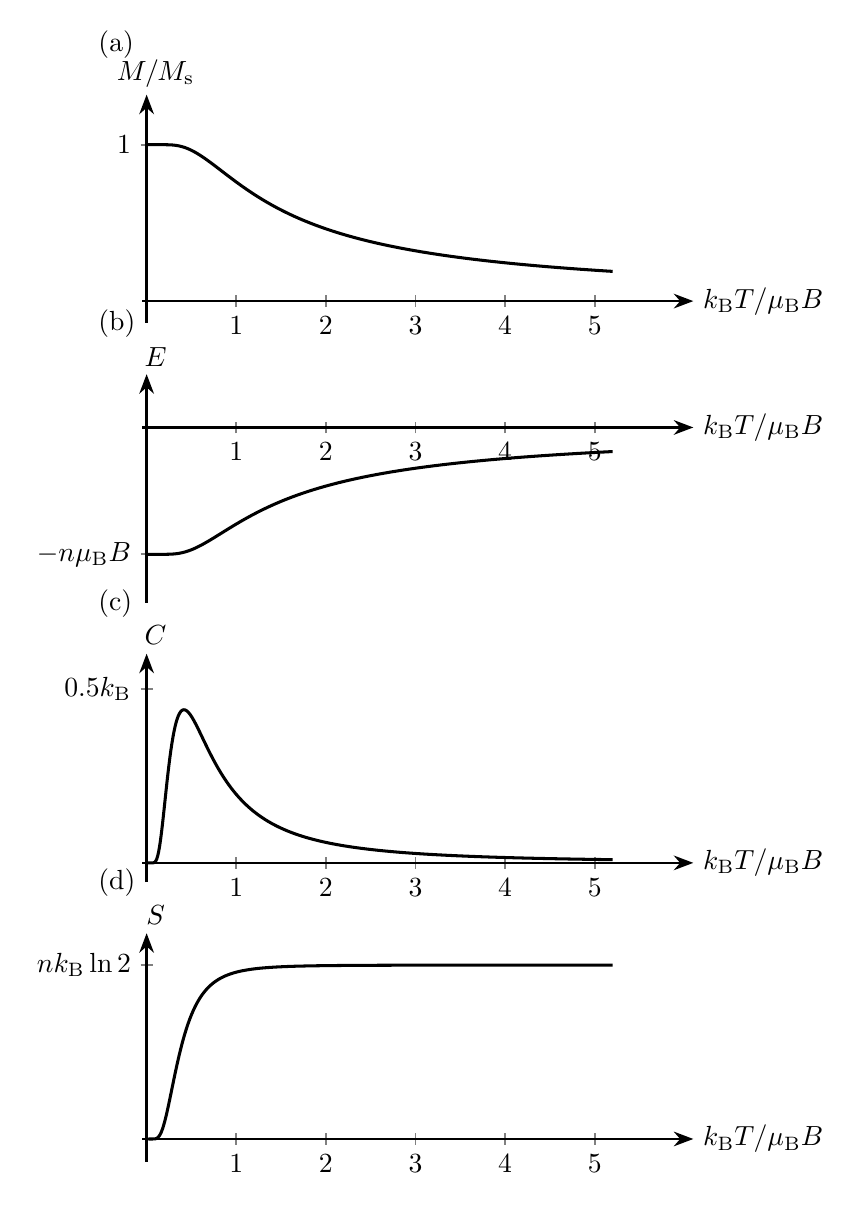
\begin{tikzpicture}[line width=0.8pt,>=Stealth]
% ---------- (a) M/Ms ----------
\begin{axis}[name=pa,at={(0cm,0cm)},anchor=north west,
  width=7.0cm,height=2.9cm,scale only axis,
  axis lines=middle,axis line style={-Stealth,line width=0.9pt},
  xmin=-0.05,xmax=6.1,ymin=-0.14,ymax=1.32,
  xtick={0,1,2,3,4,5},ytick={0,1},
  tick style={line width=0.7pt},
  xlabel={$k_{\mathrm{B}}T/\mu_{\mathrm{B}}B$},
  x label style={at={(axis cs:6.1,0)},anchor=west},
  ylabel={$M/M_{\mathrm{s}}$},
  y label style={at={(axis cs:0.1,1.33)},anchor=south,inner sep=2pt}]
  \addplot[very thick,line width=1.1pt,domain=0.01:5.2,samples=260]
    {(exp(2/x)-1)/(exp(2/x)+1)};
\end{axis}
\node[anchor=south west,inner sep=1pt] at ([xshift=-17pt,yshift=12pt]pa.north west) {(a)};
% ---------- (b) E ----------
\begin{axis}[name=pb,at={(0cm,-3.55cm)},anchor=north west,
  width=7.0cm,height=2.9cm,scale only axis,
  axis lines=middle,axis line style={-Stealth,line width=0.9pt},
  xmin=-0.05,xmax=6.1,ymin=-1.38,ymax=0.42,
  xtick={0,1,2,3,4,5},ytick={0,-1},yticklabels={0,$-n\mu_{\mathrm{B}}B$},
  tick style={line width=0.7pt},
  xlabel={$k_{\mathrm{B}}T/\mu_{\mathrm{B}}B$},
  x label style={at={(axis cs:6.1,0)},anchor=west},
  ylabel={$E$},
  y label style={at={(axis cs:0.1,0.43)},anchor=south,inner sep=2pt}]
  \addplot[very thick,line width=1.1pt,domain=0.01:5.2,samples=260]
    {-(exp(2/x)-1)/(exp(2/x)+1)};
\end{axis}
\node[anchor=south west,inner sep=1pt] at ([xshift=-17pt,yshift=12pt]pb.north west) {(b)};
% ---------- (c) C（肖特基反常） ----------
\begin{axis}[name=pc,at={(0cm,-7.1cm)},anchor=north west,
  width=7.0cm,height=2.9cm,scale only axis,
  axis lines=middle,axis line style={-Stealth,line width=0.9pt},
  xmin=-0.05,xmax=6.1,ymin=-0.055,ymax=0.60,
  xtick={0,1,2,3,4,5},ytick={0,0.5},yticklabels={0,$0.5k_{\mathrm{B}}$},
  tick style={line width=0.7pt},
  xlabel={$k_{\mathrm{B}}T/\mu_{\mathrm{B}}B$},
  x label style={at={(axis cs:6.1,0)},anchor=west},
  ylabel={$C$},
  y label style={at={(axis cs:0.1,0.61)},anchor=south,inner sep=2pt}]
  \addplot[very thick,line width=1.1pt,domain=0.01:5.2,samples=500]
    {1/(x^2*(exp(0.5/x)+exp(-0.5/x))^2)};
\end{axis}
\node[anchor=south west,inner sep=1pt] at ([xshift=-17pt,yshift=12pt]pc.north west) {(c)};
% ---------- (d) S ----------
\begin{axis}[name=pd,at={(0cm,-10.65cm)},anchor=north west,
  width=7.0cm,height=2.9cm,scale only axis,
  axis lines=middle,axis line style={-Stealth,line width=0.9pt},
  xmin=-0.05,xmax=6.1,ymin=-0.09,ymax=0.82,
  xtick={0,1,2,3,4,5},ytick={0,0.6931},yticklabels={0,$nk_{\mathrm{B}}\ln 2$},
  tick style={line width=0.7pt},
  xlabel={$k_{\mathrm{B}}T/\mu_{\mathrm{B}}B$},
  x label style={at={(axis cs:6.1,0)},anchor=west},
  ylabel={$S$},
  y label style={at={(axis cs:0.1,0.83)},anchor=south,inner sep=2pt}]
  \addplot[very thick,line width=1.1pt,domain=0.02:5.2,samples=260]
    {ln(exp(1/x)+exp(-1/x)) - (1/x)*(exp(1/x)-1)/(exp(1/x)+1)};
\end{axis}
\node[anchor=south west,inner sep=1pt] at ([xshift=-17pt,yshift=12pt]pd.north west) {(d)};
\end{tikzpicture}
\end{document}
